% % ----------------------------------------------------------------
% AMS-LaTeX Paper ***************************************
% **** -----------------------------------------------------------
\documentclass[a4paper,10pt]{beamer}
\usepackage{etex}
\setbeamertemplate{navigation symbols}{}
% \setbeamercovered{invisible}
% \addtobeamertemplate{background canvas}{\transfade[duration=0.0001]}{}
\usepackage[utf8]{inputenc}
\title{Álgebras Jacobianas asociadas a superficies a través del Lema del Diamante}
\author{Fernando Daniel Martin
\\ 
Universidad de Buenos Aires
}
\date{30/03/2016}

%%%%%%%%%%%%%%%%%%%%%%%%%%%%%%%%Mathematical packages and others%%%%%%%%%%%%%%%%%%%%%%%%%%%%%%%%%%%%%%%%%%%%%%%%%%%%%%%%%%%%%%%%%%%%%%%%%%%%%%%%%%%%%%%%%%%
\input{xy}
\xyoption{all}
\xyoption{poly}

\usepackage[all]{xy}
\usepackage{amsmath,amsthm,amsfonts,amssymb,stmaryrd}
%\usepackage[matrix,arrow]{xy}
% \usepackage{tikz-cd}
\usepackage{tikz}
\usetikzlibrary{arrows,positioning,through,decorations.pathmorphing, decorations.markings}

\usepackage{latexsym}
\usepackage{xcolor}
\usepackage{listings}
\usepackage{graphicx}%poner [dvips] para gr�ficos
\usepackage{float}  %Este packete permite controlar la flotacion de figuras al poner [H] o [h] como opcion de \begin{figure}
\usepackage [spanish]{babel}
%\usepackage{fullpage}
%\usepackage[small, bf, margin=90pt, tableposition=bottom]{caption}
%\setlength{\abovecaptionskip}{0pt}
%\usepackage[T1]{fontenc}
%\usepackage{palatino}
%\usepackage[letterpaper]{geometry}
%\geometry{top=5cm,bottom=2cm,left=3cm,right=3cm}
%\usepackage{txfonts}
\usepackage[fleqn,tbtags]{mathtools}
%\usepackage [spanish]{babel}
\usepackage{beamerthemesplit}
%\usepackage{graphics}
\usepackage{colonequals}
% \usepackage{multicol}
% \usepackage{lipsum}
\lstset{language=Python,
backgroundcolor=\color{gray!20},
numberstyle=\footnotesize,
breaklines=true,
basicstyle=\footnotesize,
keywordstyle=\bfseries\color{blue},
commentstyle=\itshape\color{purple},
%identifierstyle=\color{blue},
stringstyle=\color{orange}}

% \setlipsumdefault{1-1}
\usetheme{JuanLesPins}
%Installs the presentation theme named. Currently, the effect of this command is the same as
%saying \usepackage for the style file named beamerthemehnamei.sty for each name in the name
%list. names:boxes, Bergen, Boadilla, Madrid, AnnArbor, CambridgeUS, Pittsburgh, Rochester, Antibes, JuanLesPins, Montpellier,
%Berkeley, Ilmenau, Berlin, PaloAlto, Goettingen, Marburg, Hannover, Dresden, Darmstadt, Frankfurt, Singapore, Szeged,
%Copenhagen, Luebeck, Malmoe, Warsaw

\usecolortheme{whale}
%Same as \usetheme, only for color themes. Color style files are named beamercolorthemehnamei.sty.
%names:seahorse, rose, albatross, lily, dolphin, whale, seagull, fly, dove, crane, beetle, beaver, wolverine

%\usefonttheme[]{}
%Same as \usetheme, only for font themes. Font style files are named beamerfontthemehnamei.sty.

\useinnertheme{rounded}
%Same as \usetheme, only for inner themes. Inner style files are named beamerinnerthemehnamei.sty.
%names:circles, rectangles, rounded, innmargin; options: shadow,

\useoutertheme[hideallsubsections]{miniframes}
%Same as \usetheme, only for outer themes. Outer style files are named beamerouterthemehnamei.sty.
%names:infolines, miniframes, smoothbars, sidebars; options:footline=empty, footline=authorinstitute,
%footline=authortitle, footline=institutetitle, footline=authorinstitutetitle, subsection=(true or false)

%setbeamerfonts{title}{shape=\itshape,family=\rmfamily}
%setbeamercolor{title}{fg=red!80!black,bg=red!20!white}
\setbeamertemplate{headline}
{\begin{beamercolorbox}{section in head/foot}
\vskip2pt\insertnavigation{\paperwidth}\vskip2pt
\end{beamercolorbox}}

\setbeamertemplate{footline}
{}

\setbeamercovered{dynamic}

% ----------------------------------------------------------------
\vfuzz2pt % Don't report over-full v-boxes if over-edge is small
\hfuzz2pt % Don't report over-full h-boxes if over-edge is small

%%%%%%%%%%%%%%%%%%%%%%%%%%%%%%%%%Theorems, lemmas, corollaries, etc%%%%%%%%%%%%%%%%%%%%%%%%%%%%%%%%%%%%%%%%%%%%%%%%%%%%%%%%%%%%%%%%%%%%%%%%%%%%%%%%%%%%%%%%%
\newtheorem{teo}{Teorema}[section]
\newtheorem{coro}[teo]{Corollary}
\newtheorem{lema}[teo]{Lema}
\newtheorem{prop}[teo]{Proposici\'on}
\newtheorem{defi}[teo]{Definici\'on}%[section]
\newtheorem{obs}[teo]{Remark}%[section]
\newtheorem{rem}[teo]{Remark}
\newtheorem{notac}[teo]{Notaci\'on}
\newtheorem{ejem}[teo]{Example}
\newtheorem{por}[teo]{Porisma}
%\theoremstyle{remark}


%%%%%%%%%%%%%%%%%%%%%%%%%%%%%%%Change of names for chapters, indexes, references, etc%%%%%%%%%%%%%%%%%%%%%%%%%%%%%%%%%%%%%%%%%%%%%%%%%%%%%%%%%%%%%%%%%%%%%%
%\renewcommand{\chaptername}{Cap\'{\i}tulo}   %le asigna el nombre Cap\'{\i}tulo a Chapter
\newcommand{\invertleadsto}{\reflectbox{\,$\leadsto$\,}}%
%            \mathrel{\raisebox{.1em}{%
%            \rotatebox[origin=c]{180}{$\leadsto$}}}}
%\def\abstractname{Abstract}
\def\contentsname{\'Indice}
%\def\bibname{Referencias}   %para book
\bibliographystyle{unsrt}
\def\refname{References} %para article

%\numberwithin{equation}{section}                    %numera las ecuaciones de acuerdo a la seccion: (nn.mm)

%%%%%%%%%%%%%%%%%%%%%%%%%%%%%%Margins settings%%%%%%%%%%%%%%%%%%%%%%%%%%%%%%%%%%%%%%%%%%%%%%%%%%%%%%%%%%%%%%%%%%%%%%%%%%%%%%%%%%%%%%%%%%%%%%%%%%%%%%%%%%%%%
%\setlength{\textwidth}{7in} \setlength{\evensidemargin}{-0.25in}
%\setlength{\oddsidemargin}{-0.25in} \setlength{\textheight}{9.5in}
%\setlength{\topmargin}{-0.5in}
%\setlenght{\headheight}{16pt}

%\renewcommand\headrulewidth{.1pt}
%\fancyhead{} \fancyhead[RE]{\itshape\leftmark}
%\fancyhead[LO]{\itshape\rightmark} \fancyhead[LE,RO]{\thepage}

%\addtolength{\headheight}{17.8pt}
%30pt

%\fancyhead[LE,RO]{\footnotesize\lite\rightmark}
%\fancyfoot[C]{}
%\fancyfoot[LE,RO]{\setlength{\fboxsep}{2pt}}
%\fancyfoot[LE,RO]{\ovalbox{\footnotesize}}
%\fancyfoot[LE,RO]{\ovalbox{\itfamily}}
%\fancyfoot[LE,RO]{\ovalbox{\thepage}}
%\fancyfoot[LO,RE]{\footnotesize\itfamily\lite\title}
%\fancypagestyle{plain}{%
%\fancyhf{}
%\fancyfoot[R]{\setlength{\fboxsep}{2pt}\ovalbox{\footnotesize\sffamily\thepage}}
%\fancyfoot[L]{\footnotesize\ssfamily\lite\@title}
%\renewcommand{\headrulewidth{0pt}}
%\pagenumbering{arabic}
%\usepackage{fullpage}
%\pagestyle{headings}

%\setbeamertemplate{headline}
%

%{\usebeamercolor{palette primary}}\setbeamertemplate{sidebar canvas}[vertical shading][top=palette primary.bg,middle=white,bottom=palette primary.bg]

%%%%%%%%%%%%%%%%%%%%%%%%%%%%%%%%%Hyphenation for spanish words%%%%%%%%%%%%%%%%%%%%%%%%%%%%%%%%%%%%%%%%%%%%%%%%%%%%%%%%%%%%%%%%%%%%%%%%%%%%%%%%%%%%%%%%%%%%%

%\setcounter{tocdepth}{1}
\font\x=msbm10 scaled \magstep2

%%%%%%%%%%%Mathematical definitions in order to write less (Macros)%%%%%%%%%%%%%%%%%%%%%%%%%%%%%%%%%%%%%%%%%%%%%%%%%%%%%%%%%%%%%%%%%%%%%%%%%%%%%%%%%%%%%%%
\def\psd{\hbox{\x o}}
%\font\crest=crest

\def\id{{\mathrm{id}}}
\def\cl#1{{\langle #1 \rangle}}
\def\QED{\hfil$\Box$}
\def\qed{\begin{flushright} \QED \end{flushright}}
\def\cl#1{{\langle #1 \rangle}}

\newcommand\RR{{\mathbb{R}}}
\newcommand\QQ{{\mathbb{Q}}}
\newcommand\ZZ{{\mathbb{Z}}}
\newcommand\NN{{\mathbb{N}}}
\newcommand\CC{{\mathbb{C}}}
\newcommand\A{\mathcal{A}}
\newcommand\B{\mathcal{B}}
\DeclareMathOperator\Aut{Aut}
\DeclareMathOperator\Ext{Ext}
\DeclareMathOperator\Frac{Frac}
\DeclareMathOperator\Hom{Hom}
\DeclareMathOperator\Imw{Im}
\DeclareMathOperator\Spec{Spec}
\DeclareMathOperator\SL{SL}
\DeclareMathOperator\GL{GL}
% \DeclareMathOperator\id{id}
\newcommand\wt[1]{{(#1)}}
\newcommand\der[1]{\tfrac{\partial}{\partial#1}}
\newcommand\maxw{\mathsf{max}}
\newcommand\minw{\mathsf{min}}
\newcommand\tip{\mathsf{tip}}
\newcommand\rw{{\mathsf{R}}}
\newcommand\gldim{\mathsf{gldim}}
\newcommand\sop{\mathsf{sop}}
\DeclarePairedDelimiter\lin{\langle}{\rangle}
\DeclarePairedDelimiter\abs{\lvert}{\rvert}
\DeclarePairedDelimiter\norm{\lVert}{\rVert}
\newcommand{\kQ}{k\langle Q\rangle}
\newcommand{\KQ}{k\langle\!\langle Q\rangle\!\rangle}
\newcommand{\cyc}{\mathrm{cyc}}
\newcommand{\cf}{\mathrm{cf}}
\newcommand{\FA}{k\langle x_1,\dots,x_n\rangle}
\newcommand{\mon}{\langle X\rangle}
\newcommand{\irr}{k\langle X\rangle_{\mathrm{irr}}}
\newcommand{\llangle}{\langle\!\langle}
\newcommand{\rrangle}{\rangle\!\rangle}
% \DeclareMathSymbol{\leadsfrom}{\mathrel}{arrows}{141}
\newcommand{\Square}[2]{
\draw (-1+#1, -1+#2) to (-1+#1, 1+#2); %left vertical line
\draw (1+#1, -1+#2) to (1+#1, 1+#2); %right vertical line
\draw (-1+#1, 1+#2) to (1+#1, 1+#2); %top horizontal line
\draw (-1+#1, -1+#2) to (1+#1, -1+#2); %bottom horizontal line
}

\newcommand<>{\colorize}[4]{\only<#1>{#4}\only<#2>{\textcolor{#3}{#4}}}
% \let\pause\relax
%%%%%%%%%%%%%%%%%%%%%%%%%%%%%%%%%%%%%%%%%%%%%%%%%%%%%%%%%%%%%%%%%%%%%%%%%%%%%%%%
%%%%%%%%%%%
%%%%%%%%%%%%%%%%%%%%%%%%%%%%%%%%%%%%%%%%%%%%%%%%%%%%%%%%%%%%%%%%%%%%%%%%%%%%%%%%%%%%%%%%%%%
\begin{document}


\frame{\titlepage}
%%%%%%%%%%%%%%%%%%%%%%%%%%%%%%%%%%%%%%%%%%%%%%%%%%%%%%%%%%%%%%%%%%%%%%%%%%%%%%%%%%%%%%%%%%
% \begin{frame}
% \frametitle{Plan de la comunicaci\'on}

% \tableofcontents[pausesections,pausesubsections]

% \end{frame}
%%%%%%%%%%%%%%%%%%%%%%%%%%%%%%%%%%%%%%%%%%%%%%%%%%%%%%%%%%%%%%%%%%%%%%%%%%%%%%%%%%%%%%%%%
\section{Lema del Diamante}

\begin{frame}
 \frametitle{Motivación}
Sea $k$ un cuerpo.
\[
 A=k\langle x_1,\dots,x_n\rangle/\left(R\right).
\]

\pause
\bigskip
\begin{exampleblock}{Problema}
\begin{itemize}
\item ¿Cómo obtener una base monomial para $A$?
\item ¿Cómo llevar a un elemento de $A$ a su escritura en la base?
\end{itemize}
\end{exampleblock}

\end{frame}
\begin{frame}
\frametitle{Motivación}
\begin{exampleblock}{Ejemplo (Álgebra de Weyl)}
Sea $A=k\langle x,y\rangle/\left(yx-xy-1\right)$.

\medskip

$B=\left\{x^i y^j : i,j\in \NN_0\right\}$ es una base monomial para $A$.
\end{exampleblock}

\bigskip

\pause
Como $yx=xy+1$ en $A$, podemos reducir $yx \rightsquigarrow xy+1$ para escribir a un elemento en base $B$.

\medskip
\pause
\begin{align*}
y^2x &=y(yx)\\
 &\pause  \rightsquigarrow y(xy+1)\\&= (yx)y + y\\
&\pause \rightsquigarrow (xy+1)y + y \\&= xy^2 + 2y
\end{align*}
\end{frame}


\begin{frame}
\begin{exampleblock}{Definición}
Sea $X$ un conjunto. Un \emph{orden monomial} sobre $\langle X\rangle$ es un orden parcial $\preceq$ sobre $\langle X\rangle$ tal que:
\begin{itemize}
\item $1\preceq v$ para todo $v\in \langle X\rangle$,
\item para todo $u,v,v',w\in \langle X\rangle$, si $v\preceq v'$ entonces $uvw\preceq uv'w$.
\end{itemize}
\end{exampleblock}

\bigskip

\pause
Por ejemplo, el orden graduado lexicográfico sobre $\langle x, y, z\rangle$:
\medskip
\begin{itemize}
\item $zxy \preceq y^4$
\item $yz \preceq zy$
\end{itemize}
\end{frame}

\begin{frame}
\begin{exampleblock}{Definición}
Una \emph{regla de reescritura} en $X$ es un par $\sigma = (w_\sigma, f_\sigma) \in \langle X\rangle \times k\langle X\rangle$, con $w_\sigma \neq f_\sigma$. Notamos $w_\sigma \rightsquigarrow f_\sigma$.
\medskip

Un conjunto de reglas de reescritura se dice un \emph{sistema de reescritura}.
\end{exampleblock}

\bigskip
\pause

\begin{exampleblock}{Definición}
Dado un orden monomial $\preceq$, un sistema de reescritura $S$ es \emph{compatible} con $\preceq$ si para toda regla $w_\sigma \rightsquigarrow f_\sigma\in S$, cada monomio $u$ de $f_\sigma$ es tal que $u \preceq w_\sigma$.
\end{exampleblock}

\medskip
\pause

En el ejemplo anterior, $yx\rightsquigarrow xy+1$ es compatible con el orden graduado lexicográfico en $\langle x,y\rangle$.
\end{frame}

\begin{frame}
\begin{exampleblock}{Definición}
Supongamos que $S$ es un sistema de reescritura y $u, v, w$ son monomios de modo que existen reglas $\sigma=(uv \rightsquigarrow f_1)$ y $\tau=(vw \rightsquigarrow f_2)$ en $S$.

La 5-upla $(u,v,w,\sigma,\tau)$ es una \emph{ambigüedad} en $S$.
\end{exampleblock}

\[
\begin{tikzpicture}[scale=0.8]
\node (1) at (0,0) {$uvw$};
\node (a1) at (-2,-2) {$f_1w$};
\node (a2) at (2,-2) {$uf_2$};

\draw[->] (1) to node[above, font=\footnotesize]{} (a1);
\draw[->] (1) to node[above, font=\footnotesize]{} (a2);
\end{tikzpicture}
\]

\end{frame}

\begin{frame}
\begin{exampleblock}{Definición}
Una ambigüedad $(u,v,w,\sigma,\tau)$ en un sistema de reescritura $S$ es \emph{resoluble} si existe $f\in k\langle X\rangle$ de modo que se pueden reducir $f_1w\rightsquigarrow f$ y $uf_2\rightsquigarrow f$ aplicando reglas de reescritura en $S$.
\end{exampleblock}

\[
\begin{tikzpicture}[scale=0.8]
\node (1) at (0,0) {$uvw$};
\node (a1) at (-2,-2) {$f_1w$};
\node (a2) at (2,-2) {$uf_2$};
\node (b) at (0,-4) {$f$};

\draw[->] (1) to node[above, font=\footnotesize]{} (a1);
\draw[->] (1) to node[above, font=\footnotesize]{} (a2);
\draw[->] (a1) to node[above, font=\footnotesize]{} (b);
\draw[->] (a2) to node[above, font=\footnotesize]{} (b);
\end{tikzpicture}
\]

\end{frame}



\begin{frame}
\frametitle{El Lema del Diamante}

\begin{block}{Teorema (Lema del Diamante, Bergman -- 1978)}
Sea $X$ un conjunto, $S$ un sistema de reescritura en $X$ y $\preceq$ un orden monomial en $\langle X \rangle$ noetheriano y compatible con $S$. Sea  $I_S = (w_\sigma -f_\sigma)_{\sigma\in S}$ el ideal inducido por las reglas de $S$. Son equivalentes:
\begin{itemize}
\item Toda ambigüedad en $S$ es resoluble.
\item Los monomios $S$-irreducibles forman una base monomial para $k\langle X\rangle/I_S$.
\item Todo elemento de $k\langle X\rangle$ es de reducción única y finita para $S$.
\end{itemize}
Si estas condiciones se cumplen, el sistema $S$ es \emph{confluente}.
\end{block}

\end{frame}

\begin{frame}
Consideremos el orden graduado lexicográfico para
\[A=k[x,y,z]=k\langle x,y,z\rangle/\left(xy-yx, xz-zx, yz-zy\right).\]

\pause

El sistema 
\begin{align*}
\sigma_1&=(yx\rightsquigarrow xy),\\
\sigma_2&=(zx\rightsquigarrow xz), \\
\sigma_3&=(zy\rightsquigarrow yz)
\end{align*}
es confluente:
\[
\begin{tikzpicture}[scale=0.6]
\node (1) at (0,0) {$zyx$};
\node (a1) at (-2,-2) {$yzx$};
\node (a2) at (2,-2) {$zxy$};
\node (b1) at (-2,-4) {$yxz$};
\node (b2) at (2,-4) {$xzy$};
\node (c) at (0,-6) {$xyz$};

\draw[->] (1) to node[above, font=\footnotesize]{$\sigma_3$} (a1);
\draw[->] (1) to node[above, font=\footnotesize]{$\sigma_1$} (a2);
\draw[->] (a1) to node[left, font=\footnotesize]{$\sigma_2$} (b1);
\draw[->] (a2) to node[right, font=\footnotesize]{$\sigma_2$} (b2);
\draw[->] (b1) to node[left, font=\footnotesize]{$\sigma_1$} (c);
\draw[->] (b2) to node[right, font=\footnotesize]{$\sigma_3$} (c);
\end{tikzpicture}
\]
\pause
\[B=\left\{x^i y^jz^k : i,j,k\in \NN_0\right\}.\]
\end{frame}

% \begin{frame}
% Consideremos el orden graduado lexicográfico para
% \[A=k\langle x,y,z\rangle/\left(xy-yx, yz-zy\right).\]

% \pause

% El sistema natural es $S=\left\{\sigma_1=(yx\rightsquigarrow xy), \sigma_2=(zy\rightsquigarrow yz)\right\}$.
% \pause
% \[
% \begin{tikzpicture}[scale=0.7]
% \node (1) at (0,0) {$zyx$};
% \node (a1) at (-2,-2) {$yzx$};
% \node (a2) at (2,-2) {$zxy$};

% \draw[->] (1) to node[above, font=\footnotesize]{$\sigma_2$} (a1);
% \draw[->] (1) to node[above, font=\footnotesize]{$\sigma_1$} (a2);
% \end{tikzpicture}
% \]

% \pause
% El sistema $S$ no es confluente. Si tomamos \[S'=S\cup\left\{\sigma_3 =(zxy\rightsquigarrow yzx)\right\},\] la ambigüedad previa se resuelve, pero...
% \end{frame}


% \begin{frame}
% \[
% \begin{tikzpicture}[scale=0.7]
% \node (1) at (0,0) {$zxyx$};
% \node (a1) at (-2,-2) {$yzx^2$};
% \node (a2) at (2,-2) {$zx^2y$};

% \draw[->] (1) to node[above, font=\footnotesize]{$\sigma_3$} (a1);
% \draw[->] (1) to node[above, font=\footnotesize]{$\sigma_1$} (a2);
% \end{tikzpicture}
% \]
% \pause
% Consideremos \[S''=\left\{\sigma =(yx\rightsquigarrow xy), \tau_n=(zx^ny\rightsquigarrow yzx^n)\right\}\] donde $n\in \NN_0$. Ahora:
% \[
% \begin{tikzpicture}[scale=0.7]
% \node (1) at (0,0) {$zx^nyx$};
% \node (a1) at (-2,-2) {$yzx^{n+1}$};
% \node (a2) at (2,-2) {$zx^{n+1}y$};
% \node (b) at (0,-4) {$yzx^{n+1}$};

% \draw[->] (1) to node[above, font=\footnotesize]{$\tau_n$} (a1);
% \draw[->] (1) to node[above, font=\footnotesize]{$\sigma$} (a2);
% \draw[->] (a2) to node[right, font=\footnotesize]{$\tau_{n+1}$} (b);
% \draw[double] (a1) to (b);
% \end{tikzpicture}
% \]
% \end{frame}

\begin{frame}
\begin{exampleblock}{Heurística}
Sea $A=k\langle x_1,\dots,x_n\rangle/(r_1,\dots,r_m)$ y sea $\preceq$ el orden graduado lexicográfico.
\begin{enumerate}
\pause
\item Escribimos cada relación $r_i$ como
\[r_i = \lambda_{i,1}w_{i,1} + \lambda_{i,2} w_{i,2} + \dots + \lambda_{i,k_i} w_{i, k_i},\]
de modo que $w_{i,1}\succeq w_{i,2}\succeq\dots\succeq w_{i,k_i}$.
\pause
\item Proponemos reglas 
\[\sigma_i = w_{i,1} \rightsquigarrow -\lambda_{i,1}^{-1}\lambda_{i,2}w_{i,2}-\dots-\lambda_{i,1}^{-1}\lambda_{i,k_i}w_{i,k_i},\]
que son compatibles con $\preceq$ y tales que inducen el ideal $(r_1,\dots, r_m)$.
\pause
\item Si hay una ambigüedad $(u,v,w,\sigma,\tau)$, reducimos $uv$ y $vw$ a irreducibles $a$ y $b$; reaplicamos el proceso sobre $k\langle x_1,\dots,x_n\rangle/(r_1,\dots,r_m,a-b)$.
\end{enumerate}
\end{exampleblock}
\end{frame}

\begin{frame}
\[A=k\langle x,y,z\rangle/\left(yx-y, xz\right).\]

\pause

El sistema 
\begin{align*}
\sigma_1&=(yx\rightsquigarrow y),\\
\sigma_2&=(xz\rightsquigarrow 0)
\end{align*}
no es confluente:
\[
\begin{tikzpicture}[scale=0.6]
\node (1) at (0,0) {$yxz$};
\node (a1) at (-2,-2) {$yz$};
\node (b1) at (2,-2) {$0$};

\draw[->] (1) to node[above, font=\footnotesize]{$\sigma_1$} (a1);
\draw[->] (1) to node[above, font=\footnotesize]{$\sigma_2$} (b1);
\end{tikzpicture}
\]
\bigskip
\pause
Agreguemos la regla $\sigma_3 = (yz\rightsquigarrow 0)$.
\end{frame}

\begin{frame}
\[A=k\langle x,y,z\rangle/\left(yx-y, xz\right).\]

Ahora el sistema 
\begin{align*}
\sigma_1&=(yx\rightsquigarrow y),\\
\sigma_2&=(xz\rightsquigarrow 0),\\
\sigma_3&= (yz\rightsquigarrow 0)
\end{align*}
sí es confluente:
\pause
\[
\begin{tikzpicture}[scale=0.6]
\node (1) at (0,0) {$yxz$};
\node (a1) at (-2,-2) {$yz$};
\node (b1) at (2,-2) {$0$};
\node (c) at (0,-4) {$0$};

\draw[->] (1) to node[above, font=\footnotesize]{$\sigma_1$} (a1);
\draw[->] (1) to node[above, font=\footnotesize]{$\sigma_2$} (b1);
\draw[->] (a1) to node[below, font=\footnotesize]{$\sigma_3$} (c);
\draw[double] (b1) to node[above, font=\footnotesize]{} (c);
\end{tikzpicture}
\]
\end{frame}

\section{Álgebras Jacobianas}
\begin{frame}
\frametitle{Álgebras Jacobianas}
Sea $Q$ un quiver:
\[
\begin{tikzpicture}[->, node distance=1cm, thick, auto, scale=0.8]
\tikzstyle{every node} = [circle, fill=gray!30, minimum size=.4cm, draw=black, thin]
\tikzset{every loop/.style={looseness=15}}
\node (a) at (0:1) {};
\node (b) at (120:1) {};
\node (c) at (240:1) {};
\path (a) edge [bend right] (b)
(b) edge [bend right] (c)
(c) edge [bend right] (a)
(a) edge [in=15, out=-15, loop] (a)
(b) edge [in=135, out=105, loop] (b)
(c) edge [in=255, out=225, loop] (c);
\node (d) [right=of a,xshift=2cm] {};
\node (e) [right=of d] {};
\foreach \from/\to in {d/e, e/d}
\draw (d.40) -- (e.140);
\draw (e) -- (d);
\draw (d.320) -- (e.220);
\end{tikzpicture}
\]
\begin{exampleblock}{Definición}
Si $Q_*$ es el conjunto de caminos en $Q$, definimos el \emph{álgebra de caminos} \[\kQ=\bigoplus_{u\in Q_*} ku\] donde el producto está dado por la concatenación de caminos.
\end{exampleblock}
\end{frame}

\begin{frame}
\begin{exampleblock}{Ejemplo}
Si $Q$ es el quiver:
\[
\begin{tikzpicture}[->, thick,scale=0.8]
\tikzset{every loop/.style={looseness=15}}
\node[circle, fill=gray!30, minimum size=.4cm, inner sep=.07cm, draw=black, thin]  (1) {};
\path (1) edge [loop above] node {} (1);
\end{tikzpicture}
\]
entonces \[k\langle Q\rangle \simeq k[x]\]
\end{exampleblock}
\pause

\begin{exampleblock}{Ejemplo}
Si $Q$ es el quiver:
\[
\begin{tikzpicture}[->, auto, thick]
\tikzset{every loop/.style={looseness=15}}
\node[circle, fill=gray!30, minimum size=.5cm, inner sep=.07cm, draw=black, thin]  (1) {};
\node[circle, fill=none] (2) at +(270: 1) {...};
\path (1) edge [loop left] node {$\alpha_5$} (1);
\path (1) edge [loop above] node {$\alpha_3$} (1);
\path (1) edge [loop right] node {$\alpha_1$} (1);
\path (1) edge [in=30, out=60, loop] node {$\alpha_2$} (1);
\path (1) edge [in=210, out=240, loop] node {$\alpha_6$} (1);
\path (1) edge [in=120, out=150, loop] node {$\alpha_4$} (1);
\path (1) edge [in=300, out=330, loop] node {$\alpha_n$} (1);
\end{tikzpicture}
\]
entonces \[k\langle Q\rangle \simeq k\langle x_1,\dots,x_n\rangle\]
\end{exampleblock}
\end{frame}

\begin{frame}
En $\kQ$ hay una métrica inducida por la norma:
\[\vert x\vert =  2^{-\nu(x)}\]
donde $\nu(x)$ es el mínimo natural tal que $x$ contiene un monomio de ese grado.

\bigskip
\pause
La \emph{completación} $\KQ$ es simplemente la completación métrica de $\kQ$. Como álgebras, si $\kQ = \bigoplus A_n$ entonces $\KQ = \prod A_n$.

\medskip

Así, por ejemplo, $k\langle\!\langle \tilde{Q}\rangle\!\rangle\simeq  k\langle\!\langle x_1,\dots,x_n\rangle\!\rangle$.

\bigskip
\pause

Notar que si $(u_n)$ es una sucesión de diferentes caminos en $Q$, en $\KQ$ se tiene

\[\sum_{n=1}^k \lambda_n u_n \longrightarrow \sum_{n=1}^\infty \lambda_n u_n.\]
\end{frame}
\begin{frame}
\begin{exampleblock}{Definición}
Dado un quiver $Q$, un \emph{potencial} $P$ es una combinación lineal (posiblemente infinita) de ciclos en $\KQ$.
\end{exampleblock}
\pause

\begin{exampleblock}{Definición}
Dados un quiver con potencial $(Q,P)$, una flecha $\alpha\in Q$ y un ciclo $u=\alpha_n\dots\alpha_1$, la \emph{derivada cíclica de $u$ respecto a $\alpha$} es
\[
\partial_\alpha(u) = \sum_{k=1}^n \delta_{\alpha, \alpha_k}\alpha_{k+1}\dots\alpha_n\alpha_1\dots\alpha_{k-1}
\]
Extendiendo $\partial_\alpha$ lineal y continuamente, tenemos definido $\partial_\alpha(P)$.
\end{exampleblock}
\pause
\begin{exampleblock}{Ejemplo}
En el quiver con un único vértice y una única flecha $x$:
\[\partial_x(x^n)=\onslide<4->{nx^{n-1}}\]
\end{exampleblock}
\end{frame}

\begin{frame}
\begin{exampleblock}{Definición}
Dado un quiver con potencial $(Q,P)$, el \emph{álgebra Jacobiana asociada} es
\[J(Q,P) = \frac{\KQ}{\,\,\,\overline{\left( \partial_\alpha(P)\right)}\,\,\,}, \]
donde el índice $\alpha$ se mueve en el conjunto de flechas del quiver.
\end{exampleblock}
\pause
\bigskip
\begin{exampleblock}{Ejemplo}
Si en el quiver con un único vértice y una única flecha $x$ consideramos $P=x^n$,
\[J(Q,P) = k[x]/(x^{n-1}) \]
\end{exampleblock}
\end{frame}

\begin{frame}

\begin{block}{Teorema (Suárez-Álvarez, Vivas -- 2015)}
Sea $X$ un conjunto, $Q$ un quiver, $S$ un sistema de reescritura en $X$ y $\preceq$ un orden de caminos en $Q_*$ noetheriano en norma y compatible con $S$. Sea  $I_S = \overline{(w_\sigma -f_\sigma)}_{\sigma\in S}$ el ideal cerrado inducido por las reglas de $S$. Son equivalentes:
\begin{itemize}
\item Toda ambigüedad en $S$ es resoluble.
\item El conjunto $B$ de monomios $S$-irreducibles es tal que $\KQ/I_S\simeq k\langle\!\langle B\rangle\!\rangle$.
\item Todo elemento de $\KQ$ es de reducción única para $S$.
\end{itemize}
Si estas condiciones se cumplen, el sistema $S$ es \emph{confluente}.
\end{block}
\end{frame}

\section{Subdivisiones de superficies}
\begin{frame}
\begin{exampleblock}{Definición}
Una \emph{superficie} es una variedad diferencial sin borde, compacta, conexa, orientable y de dimensión 2.
\end{exampleblock}
\bigskip
\pause
\begin{block}{Teorema}
Las superficies están clasificadas por su \emph{género} $g\in\NN_0$:
\begin{itemize}
\item La esfera es la superficie de género 0.
\item Para $g>0$, el toro con $g$ manijas es la superficie de género $g$.
\end{itemize}
\end{block}
\end{frame}

\begin{frame}
Dada una subdivisión poligonal de una superficie $S$, construimos un quiver con potencial:
\begin{itemize}
\item En cada cara de la superficie, colocamos un ciclo orientado.
\item El potencial está dado por la suma de estos ciclos más los ciclos que rodean vértices de la subdivisión.
\end{itemize}

\pause
\bigskip
En el tetraedro:
\[
\begin{tikzpicture}[thick, scale=0.45]
\tikzstyle{every node} = [circle, fill=lightgray, minimum size=.05cm, inner sep=0cm]
\node (c) at (0,0) {};
\node (n) at (0,4) {};
\node (sw) at (210:4) {};
\node (se) at (330:4) {};
\draw[lightgray] (c) -- (sw)
	(c) -- (n)
	(c) -- (se)
	(sw) to [bend right = 45] coordinate[midway](m1) (se)
	(n) to [bend right = 45] coordinate[midway](m2) (sw)
	(se) to [bend right = 45] coordinate[midway](m3) (n);
\tikzstyle{every node} = [circle, fill=none, minimum size=.25cm, inner sep=0cm]
\node (in) at (0,2) {};
\node (isw) at (210:2) {};
\node (ise) at (330:2) {};
\node (os) at (m1) {};
\node (onw) at (m2) {};
\node (one) at (m3) {};
\draw[->, white] (in) -- (onw);
\draw[->, white] (onw) -- (isw);
\draw[->, white] (isw) -- (in);
\draw[->, white] (in) -- (ise);
\draw[->, white] (ise) -- (isw);
\draw[->, white] (ise) -- (one);
\draw[->, white] (one) -- (in);
\draw[->, white] (isw) -- (os);
\draw[->, white] (os) -- (ise);
\draw[->, white] (one) to [bend left=90, distance=100] (os);
\draw[->, white] (onw) to [bend left=90, distance=100] (one);
\draw[->, white] (os) to [bend left=90, distance=100] (onw);
\end{tikzpicture}
\]
\end{frame}

\begin{frame}
Dada una subdivisión poligonal de una superficie $S$, construimos un quiver con potencial:
\begin{itemize}
\item En cada cara de la superficie, colocamos un ciclo orientado.
\item El potencial está dado por la suma de estos ciclos más los ciclos que rodean vértices de la subdivisión.
\end{itemize}

\bigskip
En el tetraedro:
\[
\begin{tikzpicture}[thick, scale=0.45]
\tikzstyle{every node} = [circle, fill=lightgray, minimum size=.05cm, inner sep=0cm]
\node (c) at (0,0) {};
\node (n) at (0,4) {};
\node (sw) at (210:4) {};
\node (se) at (330:4) {};
\draw[lightgray] (c) -- (sw)
	(c) -- (n)
	(c) -- (se)
	(sw) to [bend right = 45] coordinate[midway](m1) (se)
	(n) to [bend right = 45] coordinate[midway](m2) (sw)
	(se) to [bend right = 45] coordinate[midway](m3) (n);
\tikzstyle{every node} = [circle, fill=black, minimum size=.25cm, inner sep=0cm]
\node (in) at (0,2) {};
\node (isw) at (210:2) {};
%\node (ise) at (330:2) {};
%\node (os) at (m1) {};
\node (onw) at (m2) {};
%\node (one) at (m3) {};
\draw[->] (in) -- (onw);
\draw[->] (onw) -- (isw);
\draw[->] (isw) -- (in);
\draw[->, white] (in) -- (ise);
\draw[->, white] (ise) -- (isw);
\draw[->, white] (ise) -- (one);
\draw[->, white] (one) -- (in);
\draw[->, white] (isw) -- (os);
\draw[->, white] (os) -- (ise);
\draw[->, white] (one) to [bend left=90, distance=100] (os);
\draw[->, white] (onw) to [bend left=90, distance=100] (one);
\draw[->, white] (os) to [bend left=90, distance=100] (onw);
\end{tikzpicture}
\]
\end{frame}

\begin{frame}
Dada una subdivisión poligonal de una superficie $S$, construimos un quiver con potencial:
\begin{itemize}
\item En cada cara de la superficie, colocamos un ciclo orientado.
\item El potencial está dado por la suma de estos ciclos más los ciclos que rodean vértices de la subdivisión.
\end{itemize}

\bigskip
En el tetraedro:
\[
\begin{tikzpicture}[thick, scale=0.45]
\tikzstyle{every node} = [circle, fill=lightgray, minimum size=.05cm, inner sep=0cm]
\node (c) at (0,0) {};
\node (n) at (0,4) {};
\node (sw) at (210:4) {};
\node (se) at (330:4) {};
\draw[lightgray] (c) -- (sw)
	(c) -- (n)
	(c) -- (se)
	(sw) to [bend right = 45] coordinate[midway](m1) (se)
	(n) to [bend right = 45] coordinate[midway](m2) (sw)
	(se) to [bend right = 45] coordinate[midway](m3) (n);
\tikzstyle{every node} = [circle, fill=black, minimum size=.25cm, inner sep=0cm]
\node (in) at (0,2) {};
\node (isw) at (210:2) {};
\node (ise) at (330:2) {};
\node (os) at (m1) {};
\node (onw) at (m2) {};
\node (one) at (m3) {};
\draw[->] (in) -- (onw);
\draw[->] (onw) -- (isw);
\draw[->] (isw) -- (in);
\draw[->] (in) -- (ise);
\draw[->] (ise) -- (isw);
\draw[->] (ise) -- (one);
\draw[->] (one) -- (in);
\draw[->] (isw) -- (os);
\draw[->] (os) -- (ise);
\draw[->] (one) to [bend left=90, distance=100] (os);
\draw[->] (onw) to [bend left=90, distance=100] (one);
\draw[->] (os) to [bend left=90, distance=100] (onw);
\end{tikzpicture}
\]
\end{frame}

\begin{frame}
Dada una subdivisión poligonal de una superficie $S$, construimos un quiver con potencial:
\begin{itemize}
\item En cada cara de la superficie, colocamos un ciclo orientado.
\item El potencial está dado por la suma de \textcolor{blue}{estos ciclos} más los ciclos que rodean vértices de la subdivisión.
\end{itemize}

\bigskip
En el tetraedro:
\[
\begin{tikzpicture}[thick, scale=0.45]
\tikzstyle{every node} = [circle, fill=lightgray, minimum size=.05cm, inner sep=0cm]
\node (c) at (0,0) {};
\node (n) at (0,4) {};
\node (sw) at (210:4) {};
\node (se) at (330:4) {};
\draw[lightgray] (c) -- (sw)
	(c) -- (n)
	(c) -- (se)
	(sw) to [bend right = 45] coordinate[midway](m1) (se)
	(n) to [bend right = 45] coordinate[midway](m2) (sw)
	(se) to [bend right = 45] coordinate[midway](m3) (n);
\tikzstyle{every node} = [circle, fill=black, minimum size=.25cm, inner sep=0cm]
\node (in) at (0,2) {};
\node (isw) at (210:2) {};
\node (ise) at (330:2) {};
\node (os) at (m1) {};
\node (onw) at (m2) {};
\node (one) at (m3) {};
\draw[->, blue] (in) -- (onw);
\draw[->, blue] (onw) -- (isw);
\draw[->, blue] (isw) -- (in);
\draw[->] (in) -- (ise);
\draw[->] (ise) -- (isw);
\draw[->] (ise) -- (one);
\draw[->] (one) -- (in);
\draw[->] (isw) -- (os);
\draw[->] (os) -- (ise);
\draw[->] (one) to [bend left=90, distance=100] (os);
\draw[->] (onw) to [bend left=90, distance=100] (one);
\draw[->] (os) to [bend left=90, distance=100] (onw);
\end{tikzpicture}
\]
\end{frame}

\begin{frame}
Dada una subdivisión poligonal de una superficie $S$, construimos un quiver con potencial:
\begin{itemize}
\item En cada cara de la superficie, colocamos un ciclo orientado.
\item El potencial está dado por la suma de \textcolor{blue}{estos ciclos} más los ciclos que rodean vértices de la subdivisión.
\end{itemize}

\bigskip
En el tetraedro:
\[
\begin{tikzpicture}[thick, scale=0.45]
\tikzstyle{every node} = [circle, fill=lightgray, minimum size=.05cm, inner sep=0cm]
\node (c) at (0,0) {};
\node (n) at (0,4) {};
\node (sw) at (210:4) {};
\node (se) at (330:4) {};
\draw[lightgray] (c) -- (sw)
	(c) -- (n)
	(c) -- (se)
	(sw) to [bend right = 45] coordinate[midway](m1) (se)
	(n) to [bend right = 45] coordinate[midway](m2) (sw)
	(se) to [bend right = 45] coordinate[midway](m3) (n);
\tikzstyle{every node} = [circle, fill=black, minimum size=.25cm, inner sep=0cm]
\node (in) at (0,2) {};
\node (isw) at (210:2) {};
\node (ise) at (330:2) {};
\node (os) at (m1) {};
\node (onw) at (m2) {};
\node (one) at (m3) {};
\draw[->] (in) -- (onw);
\draw[->] (onw) -- (isw);
\draw[->] (isw) -- (in);
\draw[->, blue] (in) -- (ise);
\draw[->] (ise) -- (isw);
\draw[->, blue] (ise) -- (one);
\draw[->, blue] (one) -- (in);
\draw[->] (isw) -- (os);
\draw[->] (os) -- (ise);
\draw[->] (one) to [bend left=90, distance=100] (os);
\draw[->] (onw) to [bend left=90, distance=100] (one);
\draw[->] (os) to [bend left=90, distance=100] (onw);
\end{tikzpicture}
\]
\end{frame}

\begin{frame}
Dada una subdivisión poligonal de una superficie $S$, construimos un quiver con potencial:
\begin{itemize}
\item En cada cara de la superficie, colocamos un ciclo orientado.
\item El potencial está dado por la suma de \textcolor{blue}{estos ciclos} más los ciclos que rodean vértices de la subdivisión.
\end{itemize}

\bigskip
En el tetraedro:
\[
\begin{tikzpicture}[thick, scale=0.45]
\tikzstyle{every node} = [circle, fill=lightgray, minimum size=.05cm, inner sep=0cm]
\node (c) at (0,0) {};
\node (n) at (0,4) {};
\node (sw) at (210:4) {};
\node (se) at (330:4) {};
\draw[lightgray] (c) -- (sw)
	(c) -- (n)
	(c) -- (se)
	(sw) to [bend right = 45] coordinate[midway](m1) (se)
	(n) to [bend right = 45] coordinate[midway](m2) (sw)
	(se) to [bend right = 45] coordinate[midway](m3) (n);
\tikzstyle{every node} = [circle, fill=black, minimum size=.25cm, inner sep=0cm]
\node (in) at (0,2) {};
\node (isw) at (210:2) {};
\node (ise) at (330:2) {};
\node (os) at (m1) {};
\node (onw) at (m2) {};
\node (one) at (m3) {};
\draw[->] (in) -- (onw);
\draw[->] (onw) -- (isw);
\draw[->] (isw) -- (in);
\draw[->] (in) -- (ise);
\draw[->, blue] (ise) -- (isw);
\draw[->] (ise) -- (one);
\draw[->] (one) -- (in);
\draw[->, blue] (isw) -- (os);
\draw[->, blue] (os) -- (ise);
\draw[->] (one) to [bend left=90, distance=100] (os);
\draw[->] (onw) to [bend left=90, distance=100] (one);
\draw[->] (os) to [bend left=90, distance=100] (onw);
\end{tikzpicture}
\]
\end{frame}

\begin{frame}
Dada una subdivisión poligonal de una superficie $S$, construimos un quiver con potencial:
\begin{itemize}
\item En cada cara de la superficie, colocamos un ciclo orientado.
\item El potencial está dado por la suma de \textcolor{blue}{estos ciclos} más los ciclos que rodean vértices de la subdivisión.
\end{itemize}

\bigskip
En el tetraedro:
\[
\begin{tikzpicture}[thick, scale=0.45]
\tikzstyle{every node} = [circle, fill=lightgray, minimum size=.05cm, inner sep=0cm]
\node (c) at (0,0) {};
\node (n) at (0,4) {};
\node (sw) at (210:4) {};
\node (se) at (330:4) {};
\draw[lightgray] (c) -- (sw)
	(c) -- (n)
	(c) -- (se)
	(sw) to [bend right = 45] coordinate[midway](m1) (se)
	(n) to [bend right = 45] coordinate[midway](m2) (sw)
	(se) to [bend right = 45] coordinate[midway](m3) (n);
\tikzstyle{every node} = [circle, fill=black, minimum size=.25cm, inner sep=0cm]
\node (in) at (0,2) {};
\node (isw) at (210:2) {};
\node (ise) at (330:2) {};
\node (os) at (m1) {};
\node (onw) at (m2) {};
\node (one) at (m3) {};
\draw[->] (in) -- (onw);
\draw[->] (onw) -- (isw);
\draw[->] (isw) -- (in);
\draw[->] (in) -- (ise);
\draw[->] (ise) -- (isw);
\draw[->] (ise) -- (one);
\draw[->] (one) -- (in);
\draw[->] (isw) -- (os);
\draw[->] (os) -- (ise);
\draw[->,blue] (one) to [bend left=90, distance=100] (os);
\draw[->,blue] (onw) to [bend left=90, distance=100] (one);
\draw[->,blue] (os) to [bend left=90, distance=100] (onw);
\end{tikzpicture}
\]
\end{frame}

\begin{frame}
Dada una subdivisión poligonal de una superficie $S$, construimos un quiver con potencial:
\begin{itemize}
\item En cada cara de la superficie, colocamos un ciclo orientado.
\item El potencial está dado por la suma de estos ciclos más los \textcolor{red}{ciclos que rodean vértices de la subdivisión}.
\end{itemize}

\bigskip
En el tetraedro:
\[
\begin{tikzpicture}[thick, scale=0.45]
\tikzstyle{every node} = [circle, fill=lightgray, minimum size=.05cm, inner sep=0cm]
\node (c) at (0,0) {};
\node[red,minimum size=.15cm] (n) at (0,4) {};
\node (sw) at (210:4) {};
\node (se) at (330:4) {};
\draw[lightgray] (c) -- (sw)
	(c) -- (n)
	(c) -- (se)
	(sw) to [bend right = 45] coordinate[midway](m1) (se)
	(n) to [bend right = 45] coordinate[midway](m2) (sw)
	(se) to [bend right = 45] coordinate[midway](m3) (n);
\tikzstyle{every node} = [circle, fill=black, minimum size=.25cm, inner sep=0cm]
\node (in) at (0,2) {};
\node (isw) at (210:2) {};
\node (ise) at (330:2) {};
\node (os) at (m1) {};
\node (onw) at (m2) {};
\node (one) at (m3) {};
\draw[->, red] (in) -- (onw);
\draw[->] (onw) -- (isw);
\draw[->] (isw) -- (in);
\draw[->] (in) -- (ise);
\draw[->] (ise) -- (isw);
\draw[->] (ise) -- (one);
\draw[->, red] (one) -- (in);
\draw[->] (isw) -- (os);
\draw[->] (os) -- (ise);
\draw[->] (one) to [bend left=90, distance=100] (os);
\draw[->, red] (onw) to [bend left=90, distance=100] (one);
\draw[->] (os) to [bend left=90, distance=100] (onw);
\end{tikzpicture}
\]
\end{frame}

\begin{frame}
Dada una subdivisión poligonal de una superficie $S$, construimos un quiver con potencial:
\begin{itemize}
\item En cada cara de la superficie, colocamos un ciclo orientado.
\item El potencial está dado por la suma de estos ciclos más los \textcolor{red}{ciclos que rodean vértices de la subdivisión}.
\end{itemize}

\bigskip
En el tetraedro:
\[
\begin{tikzpicture}[thick, scale=0.45]
\tikzstyle{every node} = [circle, fill=lightgray, minimum size=.05cm, inner sep=0cm]
\node[red,minimum size=.15cm] (c) at (0,0) {};
\node (n) at (0,4) {};
\node (sw) at (210:4) {};
\node (se) at (330:4) {};
\draw[lightgray] (c) -- (sw)
	(c) -- (n)
	(c) -- (se)
	(sw) to [bend right = 45] coordinate[midway](m1) (se)
	(n) to [bend right = 45] coordinate[midway](m2) (sw)
	(se) to [bend right = 45] coordinate[midway](m3) (n);
\tikzstyle{every node} = [circle, fill=black, minimum size=.25cm, inner sep=0cm]
\node (in) at (0,2) {};
\node (isw) at (210:2) {};
\node (ise) at (330:2) {};
\node (os) at (m1) {};
\node (onw) at (m2) {};
\node (one) at (m3) {};
\draw[->] (in) -- (onw);
\draw[->] (onw) -- (isw);
\draw[->, red] (isw) -- (in);
\draw[->, red] (in) -- (ise);
\draw[->, red] (ise) -- (isw);
\draw[->] (ise) -- (one);
\draw[->] (one) -- (in);
\draw[->] (isw) -- (os);
\draw[->] (os) -- (ise);
\draw[->] (one) to [bend left=90, distance=100] (os);
\draw[->] (onw) to [bend left=90, distance=100] (one);
\draw[->] (os) to [bend left=90, distance=100] (onw);
\end{tikzpicture}
\]
\end{frame}

\begin{frame}
Dada una subdivisión poligonal de una superficie $S$, construimos un quiver con potencial:
\begin{itemize}
\item En cada cara de la superficie, colocamos un ciclo orientado.
\item El potencial está dado por la suma de estos ciclos más los \textcolor{red}{ciclos que rodean vértices de la subdivisión}.
\end{itemize}

\bigskip
En el tetraedro:
\[
\begin{tikzpicture}[thick, scale=0.45]
\tikzstyle{every node} = [circle, fill=lightgray, minimum size=.05cm, inner sep=0cm]
\node (c) at (0,0) {};
\node (n) at (0,4) {};
\node[red,minimum size=.15cm] (sw) at (210:4) {};
\node (se) at (330:4) {};
\draw[lightgray] (c) -- (sw)
	(c) -- (n)
	(c) -- (se)
	(sw) to [bend right = 45] coordinate[midway](m1) (se)
	(n) to [bend right = 45] coordinate[midway](m2) (sw)
	(se) to [bend right = 45] coordinate[midway](m3) (n);
\tikzstyle{every node} = [circle, fill=black, minimum size=.25cm, inner sep=0cm]
\node (in) at (0,2) {};
\node (isw) at (210:2) {};
\node (ise) at (330:2) {};
\node (os) at (m1) {};
\node (onw) at (m2) {};
\node (one) at (m3) {};
\draw[->] (in) -- (onw);
\draw[->, red] (onw) -- (isw);
\draw[->] (isw) -- (in);
\draw[->] (in) -- (ise);
\draw[->] (ise) -- (isw);
\draw[->] (ise) -- (one);
\draw[->] (one) -- (in);
\draw[->, red] (isw) -- (os);
\draw[->] (os) -- (ise);
\draw[->] (one) to [bend left=90, distance=100] (os);
\draw[->] (onw) to [bend left=90, distance=100] (one);
\draw[->, red] (os) to [bend left=90, distance=100] (onw);
\end{tikzpicture}
\]
\end{frame}

\begin{frame}
Dada una subdivisión poligonal de una superficie $S$, construimos un quiver con potencial:
\begin{itemize}
\item En cada cara de la superficie, colocamos un ciclo orientado.
\item El potencial está dado por la suma de estos ciclos más los \textcolor{red}{ciclos que rodean vértices de la subdivisión}.
\end{itemize}

\bigskip
En el tetraedro:
\[
\begin{tikzpicture}[thick, scale=0.45]
\tikzstyle{every node} = [circle, fill=lightgray, minimum size=.05cm, inner sep=0cm]
\node (c) at (0,0) {};
\node (n) at (0,4) {};
\node (sw) at (210:4) {};
\node[red,minimum size=.15cm] (se) at (330:4) {};
\draw[lightgray] (c) -- (sw)
	(c) -- (n)
	(c) -- (se)
	(sw) to [bend right = 45] coordinate[midway](m1) (se)
	(n) to [bend right = 45] coordinate[midway](m2) (sw)
	(se) to [bend right = 45] coordinate[midway](m3) (n);
\tikzstyle{every node} = [circle, fill=black, minimum size=.25cm, inner sep=0cm]
\node (in) at (0,2) {};
\node (isw) at (210:2) {};
\node (ise) at (330:2) {};
\node (os) at (m1) {};
\node (onw) at (m2) {};
\node (one) at (m3) {};
\draw[->] (in) -- (onw);
\draw[->] (onw) -- (isw);
\draw[->] (isw) -- (in);
\draw[->] (in) -- (ise);
\draw[->] (ise) -- (isw);
\draw[->,red] (ise) -- (one);
\draw[->] (one) -- (in);
\draw[->] (isw) -- (os);
\draw[->,red] (os) -- (ise);
\draw[->, red] (one) to [bend left=90, distance=100] (os);
\draw[->] (onw) to [bend left=90, distance=100] (one);
\draw[->] (os) to [bend left=90, distance=100] (onw);
\end{tikzpicture}
\]
\end{frame}

\begin{frame}
\[
\begin{tikzpicture}[thick, scale=0.45]
\tikzstyle{every node} = [circle, fill=lightgray, minimum size=.05cm, inner sep=0cm]
\node (c) at (0,0) {};
\node (n) at (0,4) {};
\node (sw) at (210:4) {};
\node(se) at (330:4) {};
\draw[lightgray] (c) -- (sw)
	(c) -- (n)
	(c) -- (se)
	(sw) to [bend right = 45] coordinate[midway](m1) (se)
	(n) to [bend right = 45] coordinate[midway](m2) (sw)
	(se) to [bend right = 45] coordinate[midway](m3) (n);
\tikzstyle{every node} = [circle, fill=black, minimum size=.25cm, inner sep=0cm]
\node (in) at (0,2) {};
\node (isw) at (210:2) {};
\node (ise) at (330:2) {};
\node (os) at (m1) {};
\node (onw) at (m2) {};
\node (one) at (m3) {};
\draw[->] (in) -- (onw);
\draw[->] (onw) -- (isw);
\draw[->, red] (isw) -- (in);
\draw[->, green] (in) -- (ise);
\draw[->, red] (ise) -- (isw);
\draw[->, blue] (ise) -- (one);
\draw[->, blue] (one) -- (in);
\draw[->] (isw) -- (os);
\draw[->] (os) -- (ise);
\draw[->] (one) to [bend left=90, distance=100] (os);
\draw[->] (onw) to [bend left=90, distance=100] (one);
\draw[->] (os) to [bend left=90, distance=100] (onw);
\end{tikzpicture}
\]
\[\partial_{\textcolor{green}{\alpha}}(P) = {\textcolor{red}{x}} + {\textcolor{blue}{y}}\]
\end{frame}


\begin{frame}
\begin{exampleblock}{Definición}
El álgebra Jacobiana asociada a una subdivisión poligonal de una superficie es la inducida por el quiver con potencial que describimos.
\end{exampleblock}

\bigskip
\pause
\begin{block}{Teorema (Ladkani -- 2012)}
Supongamos que $T$ es una triangulación de una superficie.

\begin{itemize}
\item Si $T$ no es un tetraedro, el álgebra Jacobiana asociada es de dimensión finita.

\pause
\item Esto sigue siendo cierto para cualquier elección de escalares en el potencial.
\end{itemize}
\end{block}
\end{frame}

\section{Algunos resultados}
\begin{frame}
\begin{exampleblock}{Problema}
¿Qué ocurre en el tetraedro?
\end{exampleblock}

\[
\begin{tikzpicture}[thick, scale=0.45]
\tikzstyle{every node} = [circle, fill=lightgray, minimum size=.05cm, inner sep=0cm]
\node (c) at (0,0) {};
\node (n) at (0,4) {};
\node (sw) at (210:4) {};
\node (se) at (330:4) {};
\draw[lightgray] (c) -- (sw)
	(c) -- (n)
	(c) -- (se)
	(sw) to [bend right = 45] coordinate[midway](m1) (se)
	(n) to [bend right = 45] coordinate[midway](m2) (sw)
	(se) to [bend right = 45] coordinate[midway](m3) (n);
\tikzstyle{every node} = [circle, fill=black, minimum size=.25cm, inner sep=0cm]
\node (in) at (0,2) {};
\node (isw) at (210:2) {};
\node (ise) at (330:2) {};
\node (os) at (m1) {};
\node (onw) at (m2) {};
\node (one) at (m3) {};
\draw[->] (in) -- (onw);
\draw[->] (onw) -- (isw);
\draw[->] (isw) -- (in);
\draw[->] (in) -- (ise);
\draw[->] (ise) -- (isw);
\draw[->] (ise) -- (one);
\draw[->] (one) -- (in);
\draw[->] (isw) -- (os);
\draw[->] (os) -- (ise);
\draw[->] (one) to [bend left=90, distance=100] (os);
\draw[->] (onw) to [bend left=90, distance=100] (one);
\draw[->] (os) to [bend left=90, distance=100] (onw);
\end{tikzpicture}
\]
\pause
\bigskip
En el sistema de reescritura natural, aparecen 12 reglas.
\end{frame}

\begin{frame}[fragile]
\begin{lstlisting}
sage: tetra = Rewriting_System(graphs.TetrahedralGraph())
Total rules: 12
\end{lstlisting}
\pause
\begin{lstlisting}
sage: tetra.generating_function(15)
[6, 12, 12, 12, 12, 12, 12, 12, 12, 12, 12, 12, 12, 12, 12]
\end{lstlisting}
\bigskip
\pause
\begin{block}{Teorema}
El álgebra Jacobiana asociada al tetraedro es de dimensión infinita.
\end{block}
\end{frame}

\begin{frame}[fragile]
\begin{lstlisting}
sage: tetra.quiver.show()
\end{lstlisting}
\begin{figure}[h]
\centering
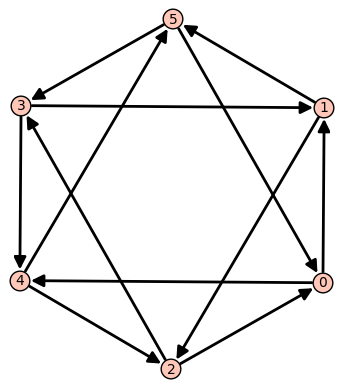
\includegraphics[scale=0.37]{tetra_quiver.png}
\end{figure}
\pause
\begin{lstlisting}
sage: tetra.rules
{(0, 2, 1): -(0, 3, 1),
 (0, 2, 4): -(0, 3, 4),
 (1, 0, 2): -(1, 5, 2),
 (1, 0, 3): -(1, 5, 3),
 (2, 1, 0): -(2, 4, 0),
 (2, 1, 5): -(2, 4, 5),
 (3, 1, 0): -(3, 4, 0),
 (3, 1, 5): -(3, 4, 5),
 (4, 0, 2): -(4, 5, 2),
 (4, 0, 3): -(4, 5, 3),
 (5, 2, 1): -(5, 3, 1),
 (5, 2, 4): -(5, 3, 4)}
\end{lstlisting}
\end{frame}

\begin{frame}
\begin{exampleblock}{Definición}
Una subdivisión poligonal de una superficie es \emph{$n$-regular} si está compuesta por polígonos de $n$ aristas, de modo que en cada vértice inciden exactamente $n$ caras.
\end{exampleblock}
\pause
\begin{exampleblock}{Ejemplos}
\begin{itemize}
\item El tetraedro es una subdivisión 3-regular de la esfera.
\pause
\item Las siguientes son subdivisiones 4-regulares del toro:
\[
\begin{tikzpicture}[scale=1.2, very thick]
%the first one of these squares wasn't actually a 4-regular subdivision,
%since its only face had 2 sides instead of 4
%\Square{-3}{0}
\Square{0}{0}
\Square{3}{0}
%\draw (-3,-1) to (-3,1);
%\draw (-4,0) to (-2,0);

\foreach \x in {-0.5,0,0.5}
{
\draw (\x, -1) to (\x, 1);
\draw (-1, \x) to (1, \x);
}

\foreach \x in {-0.75,-0.5, ..., 0.75}
{
\draw (3+\x, -1) to (3+\x, 1);
\draw (2, \x) to (4, \x);
}
\end{tikzpicture}
\]
\end{itemize}
\end{exampleblock}
\end{frame}

\begin{frame}
\begin{block}{Teorema}
El álgebra Jacobiana asociada a una subdivisión poligonal $n$-regular es de dimensión infinita.
\end{block}
\pause
\begin{block}{Idea de la demostración}
Como el ideal Jacobiano $I$ es homogéneo, tenemos una inclusión:
\begin{equation*}
\xymatrix{%
0\ar[r]&\kQ/I\ar[r]\ar@{=}[d]&\KQ/\overline I\ar@{=}[d]\\
%
0\ar[r]&\bigoplus A_n/(I\cap A_n)\ar[r]& \prod A_n/(I\cap A_n)
%
}
\end{equation*}
\pause
Basta ver que $\kQ/I$ es de dimensión infinita.
\end{block}
\end{frame}

\begin{frame}
\begin{block}{Idea de la demostración}
Los monomios que aparecen en generadores de $I$ son de la forma $(\clubsuit)$:
\begin{itemize}
\item o bien $n-1$ flechas consecutivas de la misma cara,
\item o bien $n-1$ flechas consecutivas alrededor del mismo vértice.
\end{itemize}
\pause
Si $A$ es el subespacio de $\kQ$ generado por caminos que tienen factores $(\clubsuit)$ y $B$ el generado por los que no tienen,
\[\kQ = A\oplus B.\]
\pause
Además A es un ideal, y tenemos $I\subseteq A$. Luego, para ver que $\kQ/I$ es de dimensión infinita alcanza con ver que $B$ lo es, y esto es sencillo.
\end{block}
\end{frame}

\begin{frame}
\begin{exampleblock}{Problema}
¿Existen subdivisiones $n$-regulares para $n$ arbitrariamente grande?
\end{exampleblock}
\bigskip
\pause
\begin{center}
\begin{tabular}{ c  c  c  c  c  c  c }
1 &  2 &  3 &  4 &  5 &  6 &  7\\
2 &  1 &  3 &  7 &  5 &  8 &  6\\
3 &  2 &  4 &  1 &  6 &  8 &  7\\
4 &  3 &  5 &  2 &  7 &  8 &  1\\
5 &  4 &  6 &  3 &  1 &  8 &  2\\
6 &  5 &  7 &  4 &  2 &  8 &  3\\
7 &  6 &  1 &  5 &  3 &  8 &  4\\
1 &  7 &  2 &  6 &  4 &  8 &  5
\end{tabular}
\end{center}
\end{frame}

\begin{frame}
\frametitle{Otros resultados obtenidos}
\begin{itemize}
\item Calculamos bases monomiales explícitas para las álgebras asociadas a familias de poliedros: pirámides, prismas, antiprismas.
\begin{tabular}{c c c}
      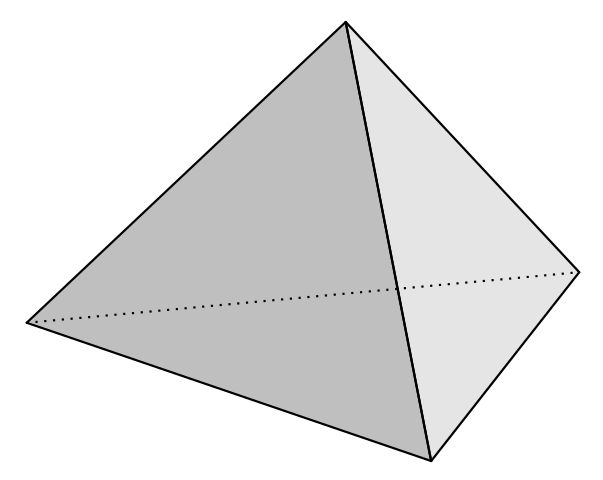
\includegraphics[width=30mm]{pyramid_p.png} &
      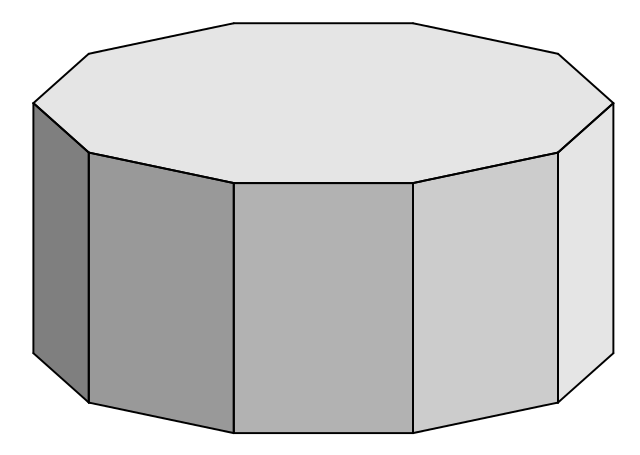
\includegraphics[width=30mm]{prism_p.png} &
      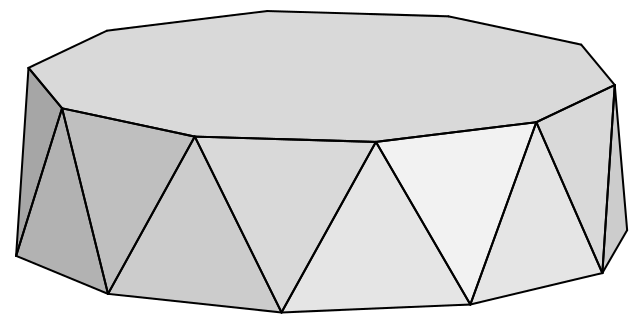
\includegraphics[width=30mm]{antiprism_p.png} 
\end{tabular}
\pause
\medskip
\item La familia de pirámides muestra que la finito-dimensionalidad del álgebra depende de la elección de escalares en el caso no triangular.
\pause
\medskip
\item Usamos las bases halladas para calcular invariantes de estas álgebras: centro y derivaciones.
\end{itemize}
\end{frame}

\begin{frame}
\frametitle{Otros resultados obtenidos}
\begin{itemize}
\item Construimos subdivisiones poligonales no triangulares con álgebra Jacobiana asociada de dimensión finita en cualquier género.
\bigskip\pause
\[
\begin{tikzpicture}[scale=0.6]
\draw (-5,1) -- (5,1);
\draw (-5,-1) -- (5,-1);

\foreach \x in {-4,-2,...,4}
\draw (\x,1) -- (\x,-1);

\foreach \x in {-4,-2,...,2}
\draw (\x,-1) -- (\x+2, 1);
\end{tikzpicture}
\]
\end{itemize}
\end{frame}

\begin{frame}
\frametitle{Otros resultados obtenidos}
\[
\begin{tikzpicture}[scale=0.5]
\draw (0,0) node[minimum size=3cm,draw] {};

\fill [black,opacity=.15] circle (2cm);

\draw[red, very thick] (-3,1) -- (-1.73,1);
\draw[red, very thick] (-3,-1) -- (-1.73,-1);

\draw[red, very thick] (3,1) -- (1.73,1);
\draw[red, very thick] (3,-1) -- (1.73,-1);

\draw[red, very thick] (1,-3) -- (1,-1.73);
\draw[red, very thick] (-1,-3) -- (-1,-1.73);

\draw[red, very thick] (1,3) -- (1,1.73);
\draw[red, very thick] (-1,3) -- (-1,1.73);

\draw[blue, very thick] (0,0) circle (2cm);
\end{tikzpicture}
\]

\[
\begin{tikzpicture}[scale=0.5]
\draw[red, very thick] (-5.44, 0.5) -- (-3.87, 0.5);
\draw[red, very thick] (-5.44, -0.5) -- (-3.87, -0.5);
\draw[red, very thick] (5.44, 0.5) -- (3.87, 0.5);
\draw[red, very thick] (5.44, -0.5) -- (3.87, -0.5);

\draw[red, very thick] (-3.5,0.87) -- (-3.5,2.7);
\draw[red, very thick] (-3.5,-0.87) -- (-3.5,-2.7);
\draw[red, very thick] (3.5,0.87) -- (3.5,2.7);
\draw[red, very thick] (3.5,-0.87) -- (3.5,-2.7);

\draw[red, very thick] (-2.137, 0.5) -- (-0.863, 0.5);
\draw[red, very thick] (-2.137, -0.5) -- (-0.863, -0.5);
\draw[red, very thick] (2.137, 0.5) -- (0.863, 0.5);
\draw[red, very thick] (2.137, -0.5) -- (0.863, -0.5);

\draw[red, very thick] (-2.5,0.87) to [bend left=40] (-0.5,0.87);
\draw[red, very thick] (2.5,0.87) to [bend right=40] (0.5,0.87);
\draw[red, very thick] (-2.5,-0.87) to [bend right=40] (-0.5,-0.87);
\draw[red, very thick] (2.5,-0.87) to [bend left=40] (0.5,-0.87);

\draw[blue, very thick] (0,0) ellipse (5.5cm and 3.5cm);
\draw[blue, very thick] (0,0) circle (1cm);
\draw[blue, very thick] (-3,0) circle (1cm);
\draw[blue, very thick] (3,0) circle (1cm);
\fill [black,opacity=.15] (-3,0) circle (1cm);
\fill [black,opacity=.15] (0,0) circle (1cm);
\fill [black,opacity=.15] (3,0) circle (1cm);
\end{tikzpicture}
\]
\end{frame}

\begin{frame}
\begin{center}
{\huge{¡Muchas gracias!}}
\end{center}
\end{frame}
\end{document}
